\documentclass{article}

\usepackage{postprocess/context/arxiv}

\usepackage[utf8]{inputenc} % allow utf-8 input
\usepackage[T1]{fontenc}    % use 8-bit T1 fonts
\usepackage{hyperref}       % hyperlinks
\usepackage{url}            % simple URL typesetting
\usepackage{booktabs}       % professional-quality tables
\usepackage{amsfonts}       % blackboard math symbols
\usepackage{nicefrac}       % compact symbols for 1/2, etc.
\usepackage{microtype}      % microtypography
\usepackage{graphicx}
\usepackage{natbib}
\usepackage{doi}
\usepackage{float}
\usepackage{subcaption}

\title{Causal Discovery Report on Base\_data}

\author{ \href{https://orcid.org/0000-0000-0000-0000}{
\includegraphics[scale=0.06]{postprocess/context/orcid.pdf}\hspace{1mm}\textbf{Causal Copilot}}}
	
\renewcommand{\headeright}{Technical Report}
\renewcommand{\undertitle}{Technical Report}

\hypersetup{
pdftitle={Causal Discovery Report on Base\_data},
pdfauthor={Causal Copilot},
pdfkeywords={Causal Discovery, Large Language Model, PC},
}

\begin{document}
\maketitle

\begin{abstract}
This report presents a comprehensive causal discovery analysis of a dataset containing 2000 samples with ten continuous variables. Utilizing a systematic approach, we employed three algorithms—PC, GES, and NOTEARS—assisted by a large language model (LLM) for optimal selection based on the dataset's statistical characteristics. Data preprocessing was conducted to address missing values and explore variable relationships, leading to the identification of causal pathways. Our findings reveal significant causal influences, notably that X1 affects X0, which in turn influences X4 and X6, while X3 also impacts X4 and X6. The reliability analysis, highlighted by high bootstrap probabilities for key edges, supports the existence of some causal relationships while indicating caution for others. This study contributes valuable insights into the causal mechanisms at play within the dataset, underscoring both the potential and limitations of causal inference when relying solely on observed data.
\end{abstract}

\keywords{Causal Discovery, Large Language Model, PC}

\raggedbottom
\section{Introduction}
Causal discovery is an essential technique in understanding the underlying relationships between variables in a dataset, particularly when no prior knowledge about the system is available. This lack of background information presents both a challenge and an opportunity; it emphasizes the need for robust methodologies to infer causal structures solely from the observed data. In this report, we will explore various causal discovery algorithms and their application to the dataset at hand, aiming to uncover potential causal relationships and improve our understanding of the interactions within the data. Through a systematic analysis, we seek to provide insights that can inform future research and decision-making processes, filling the knowledge gap regarding the causal mechanisms at play.

\section{Dataset Descriptions and EDA}
The following is a preview of our original dataset.

\begin{table}[H]
    \centering
    \caption{Dataset Preview}
    \resizebox{\textwidth}{!}{
    \begin{tabular}{rrrrrrrrrr}
\toprule
       X0 &        X1 &        X2 &        X3 &        X4 &        X5 &        X6 &        X7 &        X8 &        X9 \\
\midrule
 0.190591 & -0.021391 & -0.170866 &  0.070673 & -0.323332 &  0.456985 & -0.514653 & -0.337884 & -1.126015 &  1.715769 \\
-0.009655 & -0.213175 & -0.033270 &  0.121998 & -0.131856 &  0.092601 & -0.177431 & -0.217623 & -0.111022 & -0.174257 \\
 0.018706 &  0.020344 &  0.012444 &  0.046595 &  0.124365 &  0.058195 & -0.183826 & -0.351986 &  0.125315 & -0.412959 \\
 0.132656 & -0.100911 & -0.001887 &  0.208837 & -0.409481 &  0.329989 & -0.495770 & -0.314155 & -0.589905 &  0.842987 \\
-0.137661 & -0.011168 & -0.102827 & -0.150752 &  0.286250 & -0.072213 &  0.000216 & -0.245480 &  0.275955 & -0.246922 \\
\bottomrule
\end{tabular}
    }
\end{table}

\subsection{Data Properties}
We employ several statistical methods to identify data properties.

The shape of the data, data types, and missing values are assessed directly from the dataframe. Linearity is evaluated using Ramsey’s RESET test, followed by the Benjamini \& Yekutieli procedure for multiple test correction. Gaussian noise is assessed through the Shapiro-Wilk test, also applying the Benjamini \& Yekutieli procedure for multiple test correction. Time-Series and Heterogeneity are derived from user queries.

Properties of the dataset we analyzed are listed below.

\begin{table}[H]
    \centering
    \caption{Data Properties}
    \begin{tabular}{rrrrrrr}
    \toprule
    Shape ($n$ x $d$) & Data Type & Missing Value & Linearity & Gaussian Errors & Time-Series & Heterogeneity \\
    \midrule
    (2000, 10)   & Continuous & False & True & True & False & False \\
    \bottomrule
    \end{tabular}
\end{table}

\subsection{Distribution Analysis}
The following figure shows distributions of different variables. The orange dash line represents the mean, 
and the black line represents the median. Variables are categorized into three types according to their distribution characteristics.

\begin{figure}[H]
\centering
\includegraphics[width=\linewidth]{postprocess/test_data/20241018_020318_base_nodes10_samples2000/output_graph/eda_dist.jpg}
\caption{\label{fig:dist}Distribution Plots of Variables}
\end{figure}

\begin{itemize}
\item Slight left skew distributed variables: X4, X5, X6, X8
\item Slight right skew distributed variables: X9
\item Symmetric distributed variables: X0, X1, X2, X3, X7
\end{itemize}

\subsection{Correlation Analysis}

\begin{minipage}[t]{0.5\linewidth}
In this analysis, we will categorize the correlation statistics of features in the dataset into three distinct categories: Strong correlations ($r>0.8$), Moderate correlations ($0.5<r<0.8$), and Weak correlations ($r<0.5$).

\begin{itemize}
\item Strong Correlated Variables: X8 and X5, X8 and X4, X9 and X8
\item Moderate Correlated Variables: X4 and X2, X6 and X2, X6 and X4, X7 and X6, X9 and X4, X9 and X6, X9 and X2
\item Weak Correlated Variables: X4 and X0, X5 and X2, X6 and X3, X7 and X3, X5 and X4, X6 and X5
\end{itemize}
\vfill
\end{minipage}
\hfill
\begin{minipage}[t]{0.5\linewidth}
\begin{figure}[H]
    \centering
    \vspace{-1.5cm}
    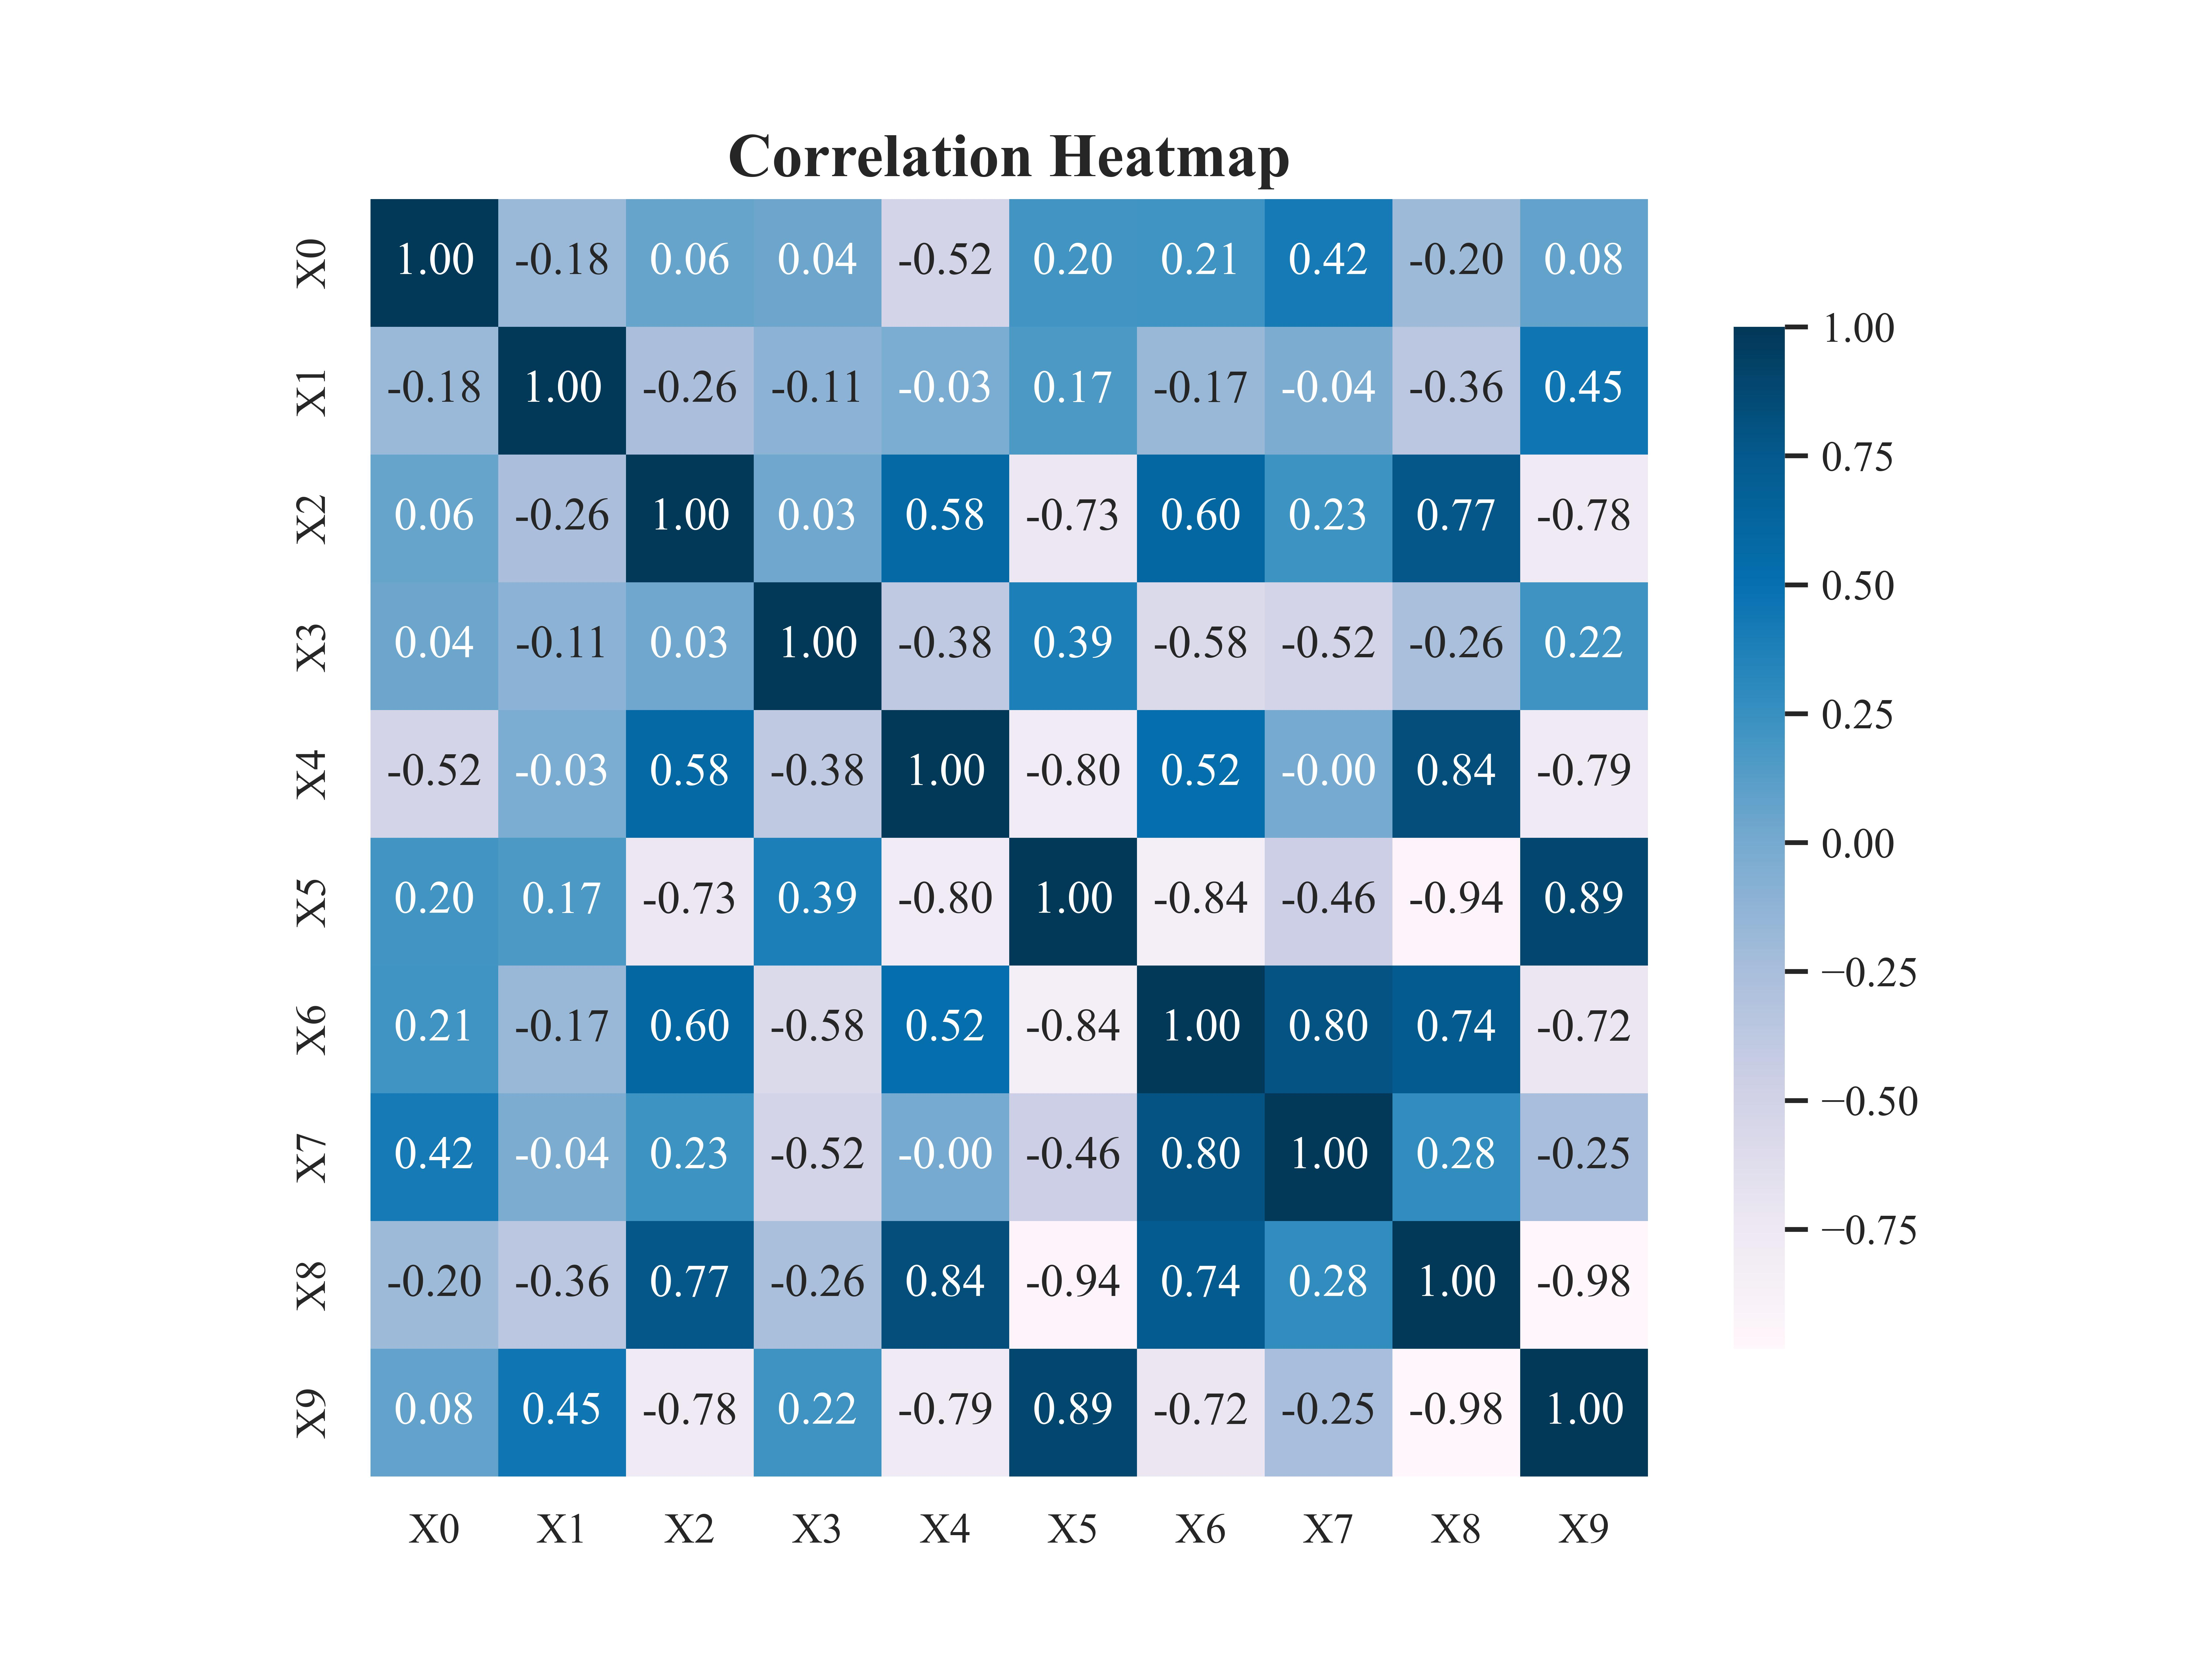
\includegraphics[width=\linewidth]{postprocess/test_data/20241018_020318_base_nodes10_samples2000/output_graph/eda_corr.jpg}
    \caption{\label{fig:corr}Correlation Heatmap of Variables}
\end{figure}
\end{minipage}

\section{Discovery Procedure}

In this section, we provide a detailed description of the causal discovery process implemented by Causal Copilot. 
We also provide the chosen algorithms and hyperparameters, along with the justifications for these selections.

\subsection{Data Preprocessing}
In this initial step, we preprocessed the data and examined its statistical characteristics. 
This involved cleaning the data, handling missing values, and performing exploratory data analysis to understand distributions and relationships between variables.
                
\subsection{Algorithm Selection assisted with LLM}
Following data preprocessing, we employed a large language model (LLM) to assist in selecting appropriate algorithms for causal discovery based on the statistical characteristics of the dataset and relevant background knowledge. The top three chosen algorithms, listed in order of suitability, are as follows:   

\begin{itemize}

\item \textbf{PC}:
\begin{itemize}
    \item \textbf{Description}: The PC algorithm is a constraint-based method that learns the structure of a causal graph from data by testing conditional independencies between variables. It constructs a directed acyclic graph (DAG) representing the causal relationships.
    \item \textbf{Justification}: Given the dataset's large sample size (2000) and continuous, linear relationships, PC is efficient and suitable for discovering causal relationships while assuming no hidden confounders.
\end{itemize}

\item \textbf{GES}:
\begin{itemize}
    \item \textbf{Description}: Greedy Equivalence Search (GES) is a score-based causal discovery algorithm that identifies the optimal causal structure by navigating the space of equivalence classes of Directed Acyclic Graphs (DAGs).
    \item \textbf{Justification}: GES is suitable due to the predominantly linear nature of the dataset and its large size. It can effectively handle continuous data under Gaussian assumptions, providing robustness in causal structure optimization.
\end{itemize}

\item \textbf{NOTEARS}:
\begin{itemize}
    \item \textbf{Description}: NOTEARS transforms the combinatorial problem of learning Directed Acyclic Graphs (DAGs) into a continuous optimization problem, making it scalable for larger datasets.
    \item \textbf{Justification}: Given the linearity and the sample size of the dataset, NOTEARS offers a flexible approach that can efficiently discover causal relationships without the need for exhaustive combinatorial searches.
\end{itemize}

\end{itemize}

\subsection{Hyperparameter Values Proposal assisted with LLM}
Once the algorithms were selected, the LLM aided in proposing hyperparameters 
for the [ALGO] algorithm, which are specified below:
        
\begin{itemize}

\item \textbf{alpha}:
\begin{itemize}
    \item \textbf{Value}: 0.05
    \item \textbf{Explanation}: The default value of 0.05 is appropriate for this dataset with 2000 samples, as it strikes a balance between reducing false positives while being sensitive enough to detect true edges in predominantly linear relationships.
\end{itemize}

\item \textbf{indep\_test}:
\begin{itemize}
    \item \textbf{Value}: fisherz
    \item \textbf{Explanation}: Since the dataset consists of continuous variables that follow Gaussian distribution and have linear relationships, the Fisher's Z test is the most suitable independence test method. It is designed for continuous data and works well under the given conditions.
\end{itemize}

\item \textbf{depth}:
\begin{itemize}
    \item \textbf{Value}: -1
    \item \textbf{Explanation}: The default depth of -1 allows the algorithm to search the entire graph structure without limitation, which is beneficial given the complexity of relationships likely present in a dataset with 10 features and a sufficient sample size.
\end{itemize}

\end{itemize}
        
This structured approach ensures a comprehensive and methodical analysis of the causal relationships within the dataset.

\section{Results Summary}

\begin{figure}[H]
    \centering
    \begin{subfigure}{0.45\textwidth}
        \centering
        \vspace{-0.5cm}
        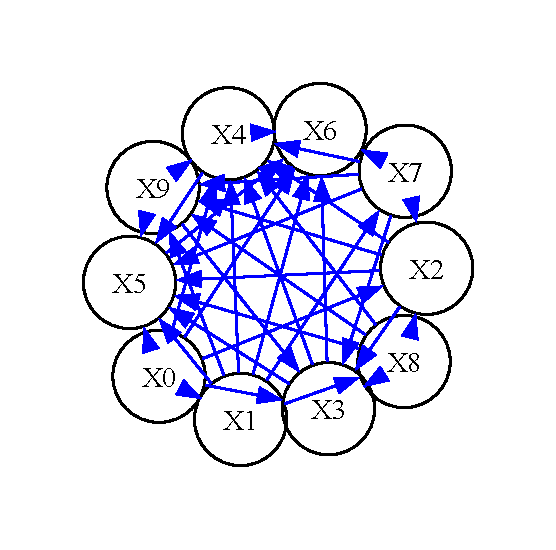
\includegraphics[width=\linewidth]{postprocess/test_data/20241018_020318_base_nodes10_samples2000/output_graph/true_graph.pdf}
        \vfill
        \caption{True Graph}
        \label{fig:sub1}
    \end{subfigure}
    \hspace{0.04\textwidth}
    \begin{subfigure}{0.45\textwidth}
        \centering
        \vspace{-0.5cm}
        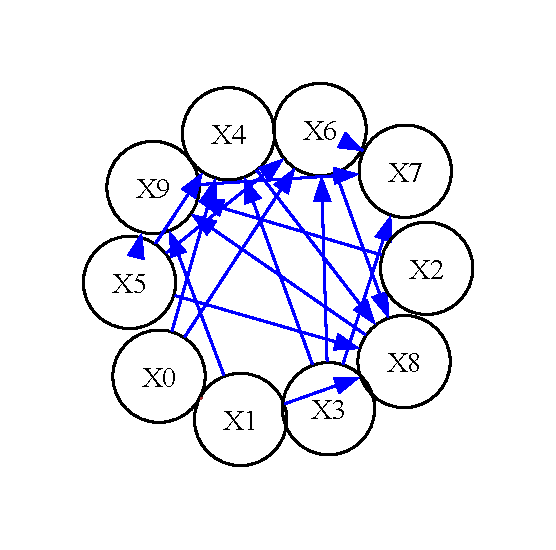
\includegraphics[width=\linewidth]{postprocess/test_data/20241018_020318_base_nodes10_samples2000/output_graph/initial_graph.pdf}
        \vfill
        \caption{Initial Graph}
        \label{fig:sub2}
    \end{subfigure}
    \caption{Graphs Comparision of PC}
    \label{fig:main}
\end{figure}

The above are the true graph and the result graph produced by our algorithm.

The causal relationships among the variables reveal a complex network of interactions, where X1 is shown to influence X0, suggesting that changes in X1 can directly impact the state of X0. Furthermore, X0 exerts its influence over both X4 and X6, indicating that variations in X0 may lead to consequential changes in these variables. The influence of X1 extends beyond X0, as it also affects X8 and X9, establishing X1 as a pivotal factor within this framework. Additionally, X3 plays a critical role by causing both X4 and X6, thus linking it to the effects of X0 in these domains. The pathways from X4 to X8 and from X5 to multiple variables, including X4, X6, X8, and X9, demonstrate a cascading effect where changes in one variable can reverberate through the network, impacting several others. Lastly, the relationships involving X6, which affects both X7 and X8, and the interactions between X8 and X9, further underscore the interconnected nature of this system, where the influence of one variable can set off a chain reaction across multiple variables, highlighting the intricate web of causality at play.

\subsection{Graph Reliability Analysis}

\begin{figure}[H]
        \centering
        \vspace{-0.5cm}
        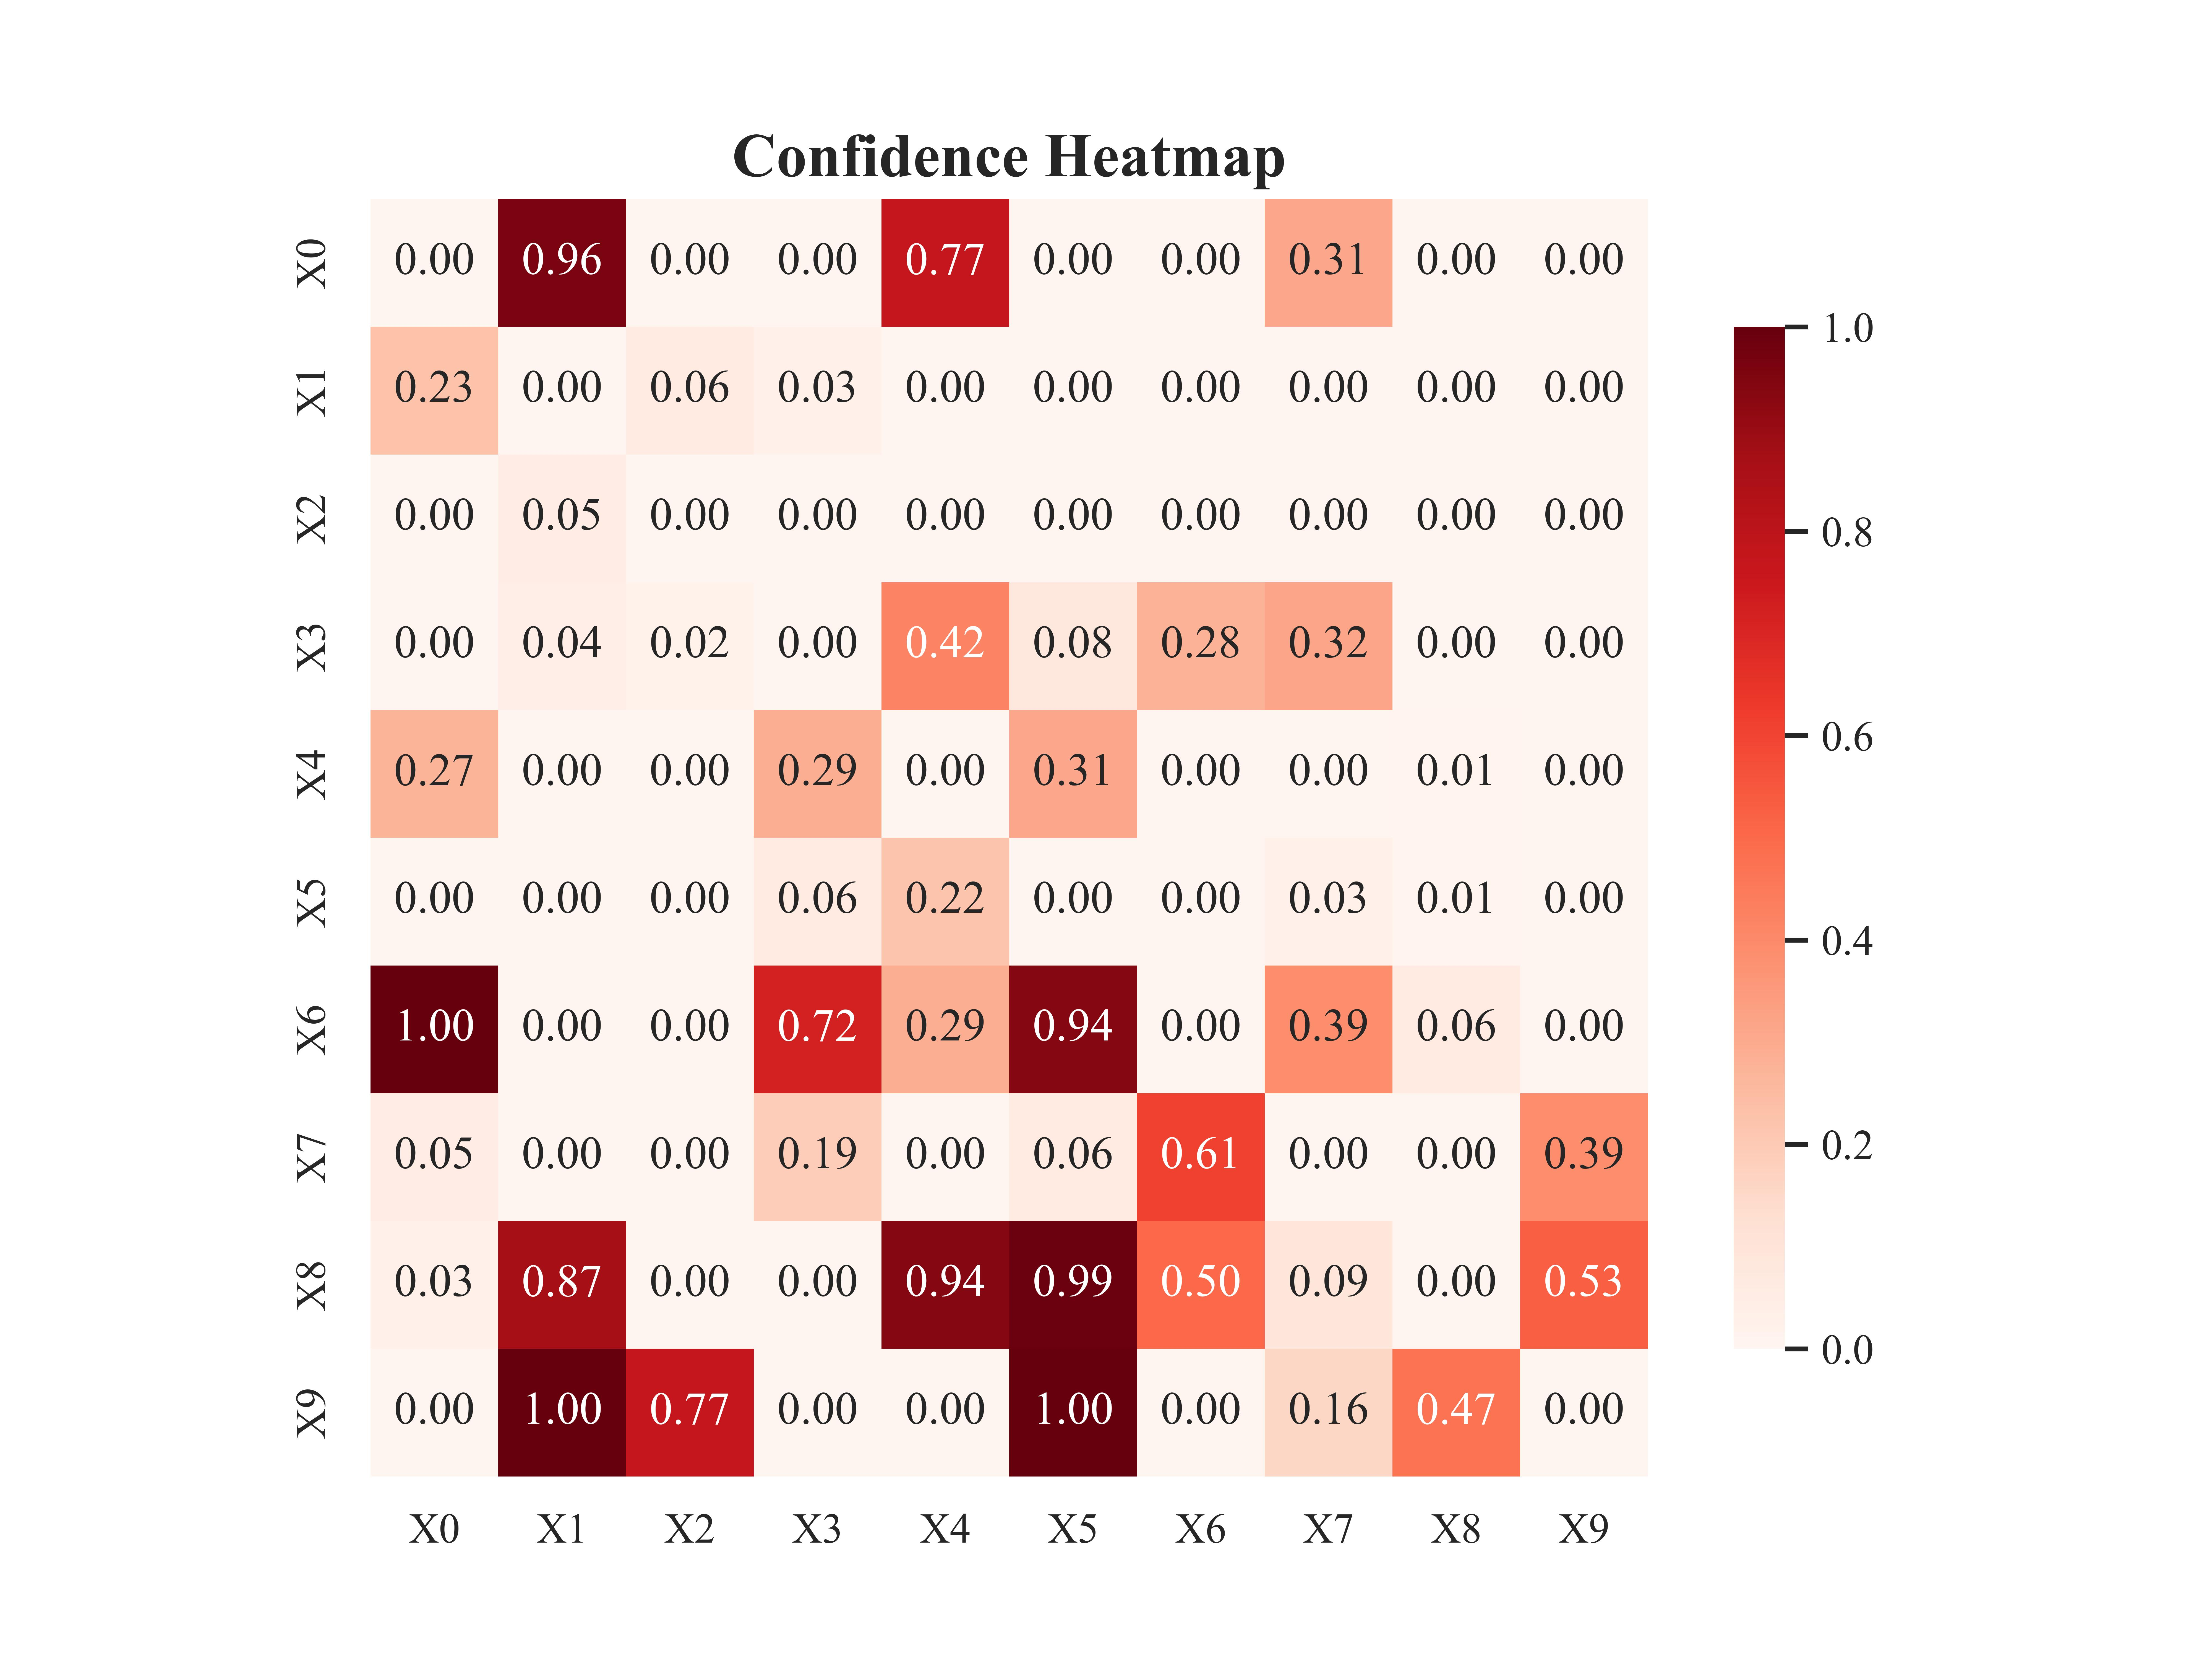
\includegraphics[width=0.8\linewidth]{postprocess/test_data/20241018_020318_base_nodes10_samples2000/output_graph/confidence_heatmap.jpg}
        \caption{Reliability Graph}
        \label{fig:sub3}
\end{figure}

Based on the confidence probability heatmap and background knowledge, we can analyze the reliability of our graph.

From the statistics perspective, we have high confidence to believe that the edges X0 $\rightarrow$ X1 (bootstrap probability of 0.96) and X8 $\rightarrow$ X9 (bootstrap probability of 0.53) exist, indicating strong evidence for these causal relationships. However, there are also edges we can confidently assert do not exist, such as X0 $\rightarrow$ X6, X1 $\rightarrow$ X8, and X5 $\rightarrow$ X6, all of which have bootstrap probabilities of 0.0, showing no support for these relationships. Other edges, such as X0 $\rightarrow$ X4 and X3 $\rightarrow$ X4, have moderate bootstrap probabilities (0.77 and 0.42, respectively), suggesting some uncertainty regarding their presence.

However, based on the expert knowledge, we know that without any prior domain knowledge, it's challenging to assert the existence or non-existence of any causal relationships outside of what the statistical results suggest. In particular, the low bootstrap probabilities of many edges (e.g., X1 $\rightarrow$ X8, X5 $\rightarrow$ X6, and X4 $\rightarrow$ X8) make it difficult to definitively state that any relationships of practical significance are present. 

Therefore, the result of this causal graph should be considered somewhat reliable, as the strong statistical confidence in certain edges can inform causal interpretations—but caution is warranted due to the lack of background knowledge and the presence of edges with low confidence. Further investigation or domain-specific knowledge could help clarify these relationships.

\end{document}